%%%%%%%%%%%%%%%%%%%%%%%%%%%%%%%%%%%%%%%%%%%%%%%%%%%%%%%%%%%%%%%%%%%%%%%%%%%%%%%%%%%%%%%%%%%%%%%%%%
%% This file contains a description of the UI and functionality for the editor portion of the GUI.
%% Trevor Morse
%% CS 383
%% 10/31/2016
%%%%%%%%%%%%%%%%%%%%%%%%%%%%%%%%%%%%%%%%%%%%%%%%%%%%%%%%%%%%%%%%%%%%%%%%%%%%%%%%%%%%%%%%%%%%%%%%%%

%TODO: adjust header info as necessary to mesh with spec.tex and other child documents
\usepackage{graphicx}

\begin{document}
	\section{Editor}
	
	\subsection{Mock-up}
	\begin{figure}[!htb]
		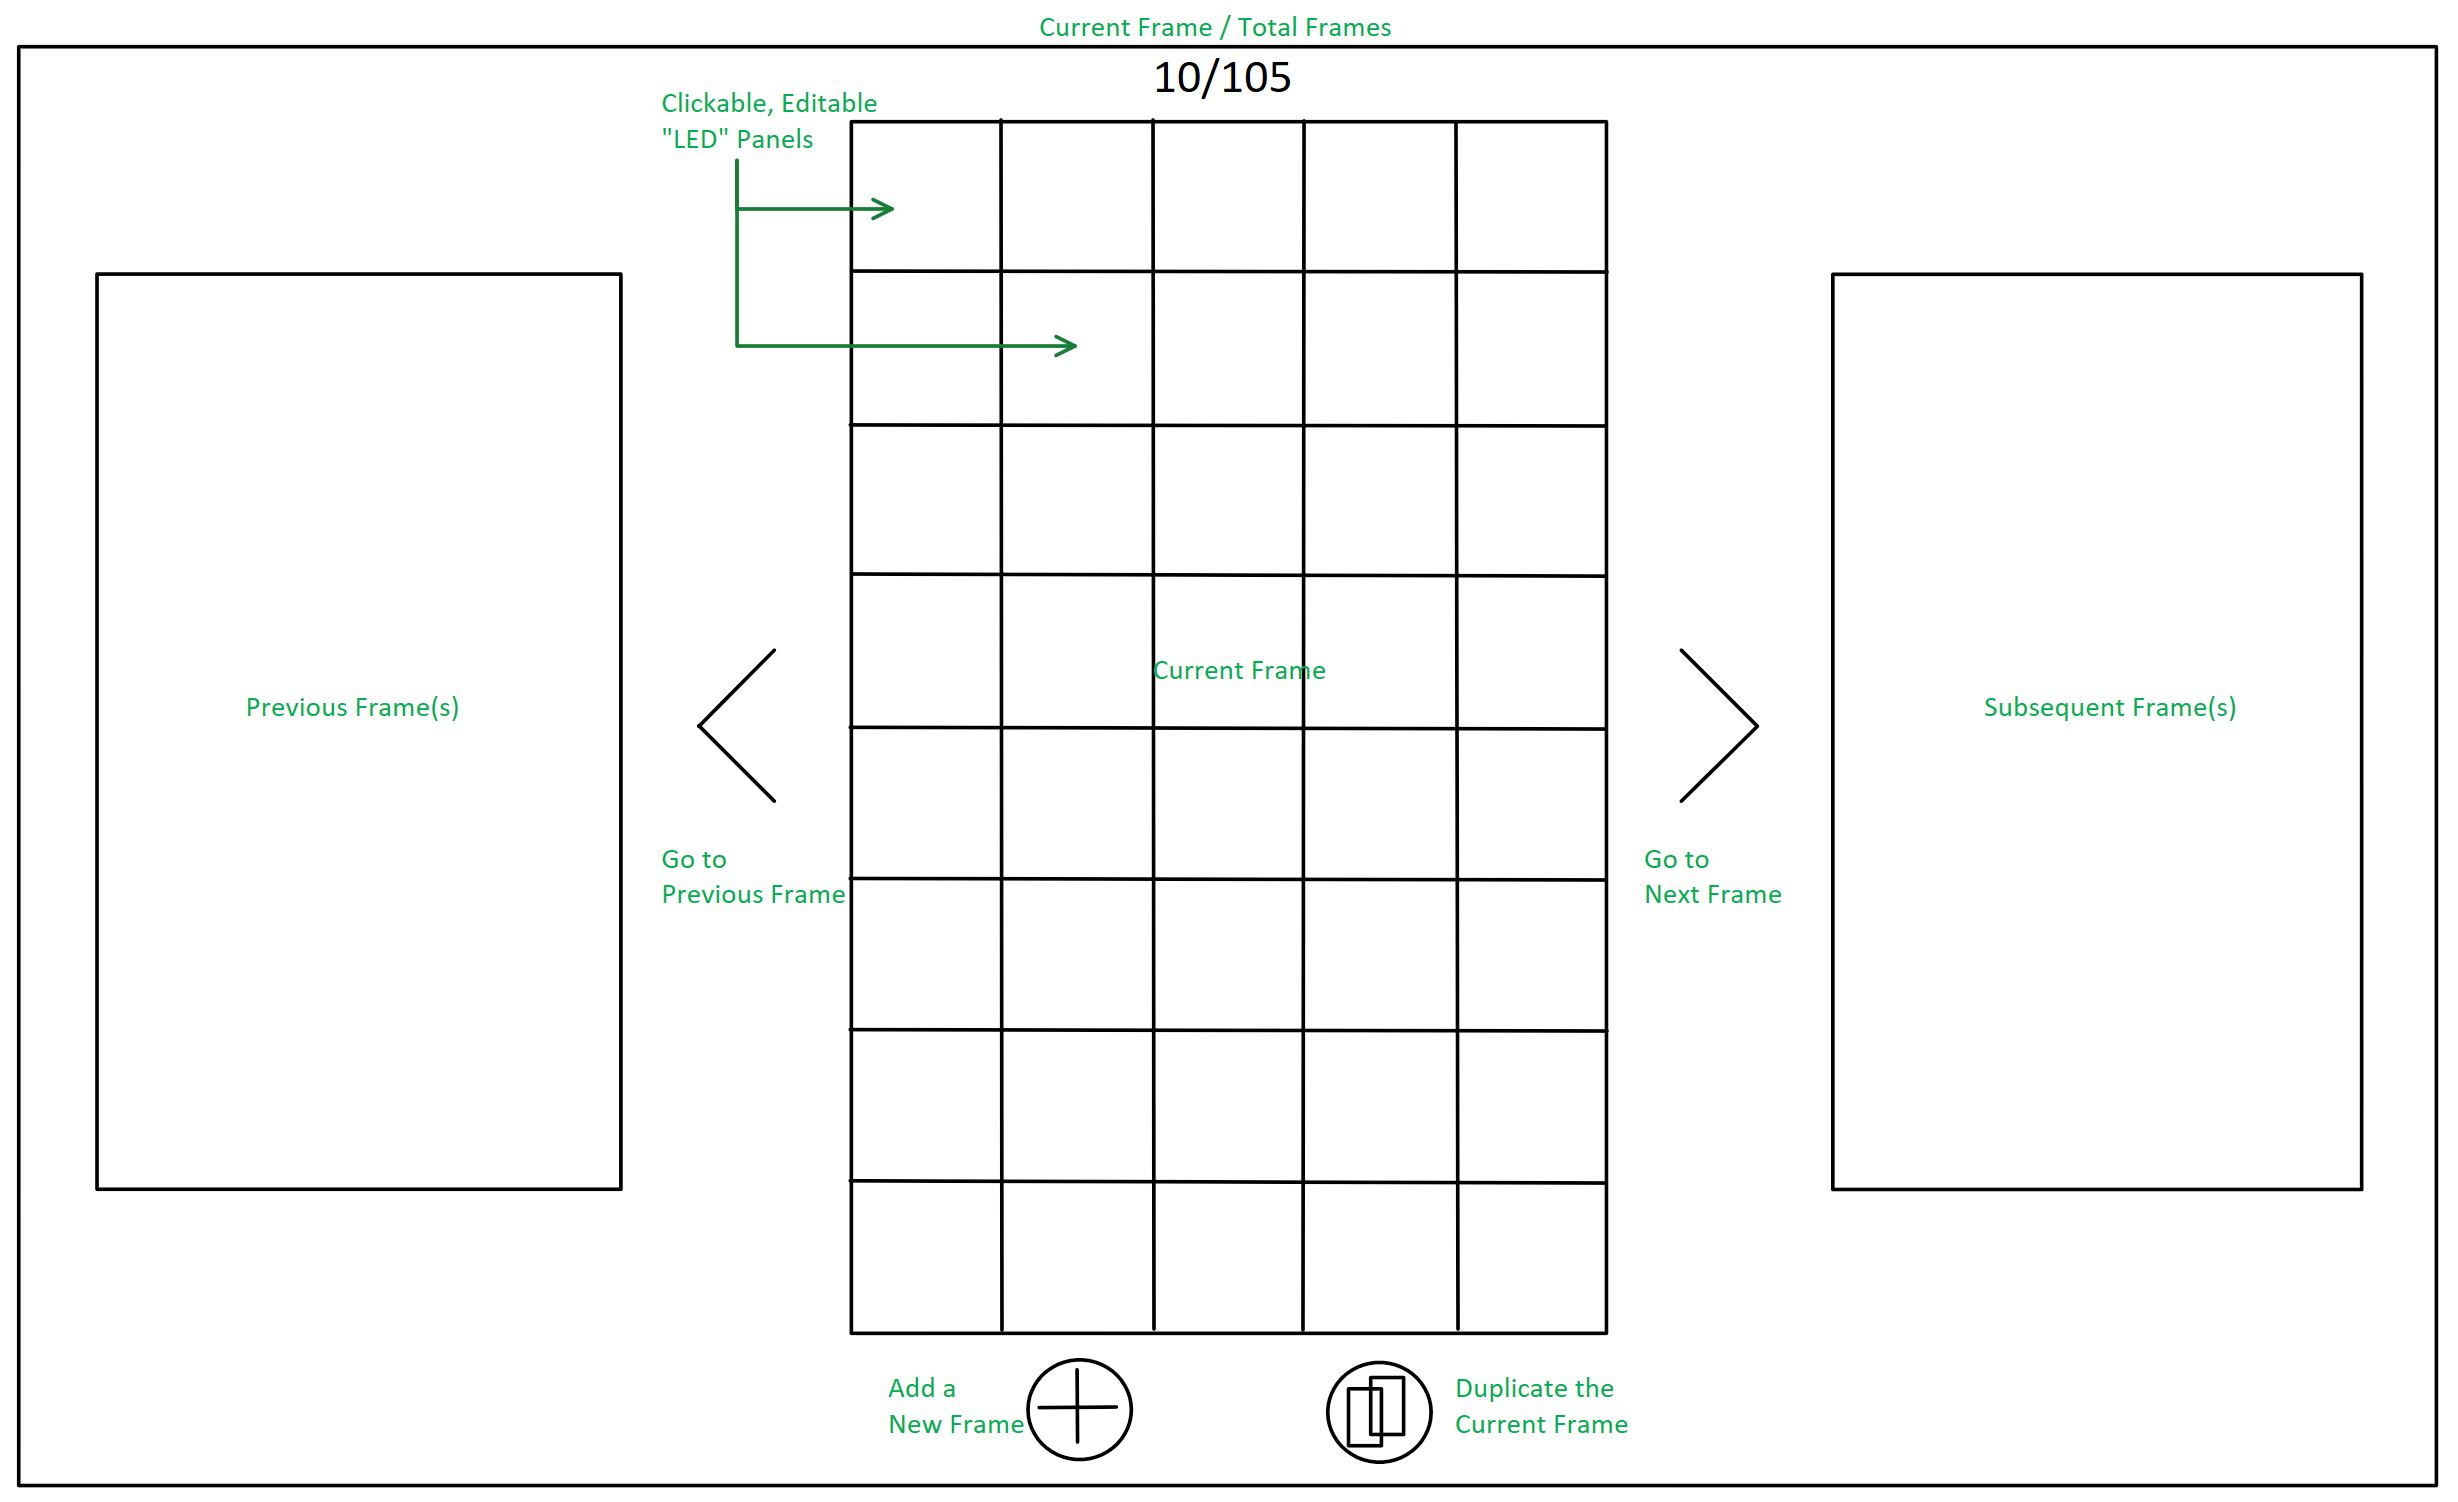
\includegraphics[width=\linewidth]{../mockups/editor_view.jpg}
		\caption{Initial Mock-up of the editor section of the GUI.}
		\label{fig:editor_view}
	\end{figure}
	
	\subsection{Functionality}
	The following descriptions reference Figure \ref{fig:editor_view} above.
	\begin{itemize}
		\item This section of the GUI is the primary area for editing a frame within the overall animation. The primary focus is on the current frame in the center of the view, with smaller references to the previous and subsequent frames to the sides.
		\item Navigation:
		\begin{itemize}
			\item Above the current frame, there is an indicator of the current position relative to the total number of frames.
			\item In order to navigate to a previous or subsequent slide, the user will be able to click on the arrows to the sides of the current frame.
			\item Possible Addition: Mini-frame representations surrounding the numbers indicating the position of the frame. These could allow for speedy navigation across a large number of frames.
		\end{itemize}
		\item Editing:
		\begin{itemize}
			\item In order to edit a given frame, the user will utilize a combination of features in this section as well as in the toolboxes. %TODO: reference the Toolbox section here
			\item The current frame will be enlarged in the center of the view. Each panel inside represents an LED panel on the tower (panels in the figure are not necessarily to scale).
			\item The user will be able to select one or more LED panels at a time and specify the given options within the toolboxes.
			\item Below the current frame are two buttons. One allows the user to insert a new, blank frame immediately after the current frame. The other button allows the user to duplicate the current frame in a new frame after it.
		\end{itemize}
	\end{itemize}
	
	\subsection{Notes}
	\begin{itemize}
		\item The editor section of the GUI will work alongside the toolboxes. These toolboxes will display to the left of the editor. They will provide options for editing a particular LED panel and/or overall frame. %TODO: reference the Toolbox section here
		\item There will also be options in the GUI's menus that will help with more efficient editing and navigation of frames.
		\item The plan is to develop the UI of the editor first to help solidify the design. Once the design has been solidified, more in-depth functionality will be added.
	\end{itemize}
	
\end{document}